\documentclass[10pt,twocolumn,letterpaper]{article}

\usepackage{ae}%
\usepackage{amsmath}
\usepackage{cvpr}
\usepackage{times}
\usepackage{epsfig}
\usepackage{graphicx}
\usepackage{amsmath}
\usepackage{amssymb}
\usepackage[utf8]{inputenc}


\usepackage[breaklinks=true,bookmarks=false]{hyperref}

\cvprfinalcopy % *** Uncomment this line for the final submission

\def\cvprPaperID{****} % *** Enter the CVPR Paper ID here
\def\httilde{\mbox{\tt\raisebox{-.5ex}{\symbol{126}}}}

\setcounter{page}{1}
\begin{document}

%%%%%%%%% TITLE
\title{\ MÉTODOS DE SEGMENTACIÓN}

\author{K. Guarin \\
University of Los Andes\\
{\tt\small gk.guarin10@uniandes.edu.co}
% For a paper whose authors are all at the same institution,
% omit the following lines up until the closing ``}''.
% Additional authors and addresses can be added with ``\and'',
% just like the second author.
% To save space, use either the email address or home page, not both
}
\maketitle
%\thispagestyle{empty}
%%%% %%%%% ABSTRACT
\begin{abstract}
 La segmentación de imágenes juega un papel muy importante en visión artificial o visión por computador, donde los objetivos principales son poder crear súper píxeles para extraer objetos hasta llegar a satisfacer las necesidades o metas del observador.
 Hasta el día de hoy se han estudiado diferentes métodos en los que se incluyen el agrupamiento de las imágenes digitales, ya sea mediante la utilización de clúster que asocian semejanzas de los píxeles o mediante la jerarquía estimando con el nivel de gris,
 tono o luminancia interpretado como la altitud del relieve en una imagen. En este trabajo se realizó la implementación de 3 técnicas de segmentación de imágenes digitales, utilizando diferentes espacios de color por último se evaluaron los métodos propuesto
 y se compararon métodos avanzados encontrando que .

   {\bf Palabras clave:} segmentación, k-means, gmm, watershed, hsv, lab, ucm.
   
   \end{abstract}

%%%%%%%%% BODY TEXT
\section{Introducción}

La visión artificial como ciencia de la computación engloba diferentes técnicas para el procesamiento digital de imágenes buscando día a día que los 
computadores puedan interpretar las imágenes como las perciben los seres humanos. Con el enorme momento del big data y la diversidad de aplicaciones 
en las que es necesario el uso de imágenes, es posible evidenciar como el estudio de diferentes técnicas de segmentación y en general de procesamiento
de imágenes se ha acrecentado.Los algoritmos de segmentación generalmente se basan en el análisis y procesamiento de una de dos propiedades básicas de
los valores de intensidad: la discontinuidad(cambios abruptos en la intensidad) y similitud (regiones similares según un conjunto de criterios predefinidos).
La segmentación de imágenes significa subdividir en regiones u objetos para permitir de una u otra forma “mejorar” una imagen para posteriormente ser analizada a 
profundidad y poder comprender los objetos en el campo de visión. 
\\
\\
En la actualidad se han desarrollado diferentes métodos de segmentación para la reconstrucción 3D de modelos anatómicos a partir de técnicas de clustering  
A continuación se enuncian 3 métodos de segmentación.\cite{RODRIGUEZ1997} 
dos aplicaciones más 
\\
\\
\\
Introducción a mi proyecto 


\subsection{Métodos}
\textbf{K-means}
\\
Es una de las técnicas de agrupamiento más simples usadas en la segmentación de datos e imágenes, cuyo objetivo principal es dividir elementos en grupos o clusters, donde cada
elemento del grupo es similar a otro elemento del mismo grupo.El centroide es el valor o vector característico de cada grupo y representa el “centro” del grupo, dado que los
grupos generalmente tienen forma circular.
\begin{equation}\label{eq:1}
\sum_{i=0}^k \sum_{x_j\in S_i}||x_{i}-u_{i}||^2 
\end{equation}
\newline
\\
$Algoritmo:$
\begin{enumerate}
\item Seleciona el número de grupos.
\item Asigna elementos a cada cluster.
\item Computa nuevos centroides.
\item Itera hasta optener una estabilidad en las asignaciones.
\end{enumerate}

\textbf{Gmm}
\\
Técnica basada en la representación de cada grupo como una distribución gaussiana; los clúster son formados por la representación de la función de densidad de probabilidad.
La distancia de un punto a otro está dada por el cálculo de la distancia de Mahalanobis, lo cual permite que la distancia se adapte a la distribución de los datos. 
\newline
\\
\begin{equation}
 \sum_{k} \pi_{k}\frac{1}{\sum_k} e^{-d(x,\mu_k;\sum_k)}
\end{equation}
$Algoritmo:$
\begin{enumerate}
\item Seleccionar el número de grupos.
\item Asigna una densidad de probabilidad por grupo.
\item Calcula la distancia euclidiana.
\item Asigna responsabilidades a cada punto.
\item Itera hasta converger a un mínimo local.
\end {enumerate}

\textbf{Watershed}
\newline
Es una técnica de segmentación inspirada en las cuencas hidrográficas, donde la cuenca representa
el conjunto de puntos en los que todas las gotas de lluvia convergen a la misma ubicación. 
las líneas del watershed separan dos cuencas.
En imágenes el tono se interpreta como la altitud de relieve en una imágen y para calcular las cuencas 
se toman los mínimos regionáles y se realiza la inundación hasta el nivel deseado.
\newline
\\
$Algoritmo$

\begin{enumerate}
 \item Se hace un agujero para cada mínimo regional de la superficie topográfica.
 \item Se sumerje en agua poco a poco la superficie.
 \item Se van formando lagos y cuando los lagos se encuentran se ubica una línea para evitar que los dos lagos se unan.
 \item El conjunto de presas de agua son las cuencas. 
 \end{enumerate}

inicia con la subdivisión disminuida por la fusió de las 
cuencas hidrográficas. e elementos básicos de volumen,
topologicamente se le llama cuenca a la magnitud del gradiente minuída   


\subsection{Espacios de color}

rgb: modelo basado en la sitesis aditiva con el que es posible representar 
un color mediante la mezcla por adicion de los 3 colores primarios cian, magenta, amarillo 
y negro y 3 componentes espectrales primarias (rojo verde azul)

hsv: se define como color en terminos de sus componentes. 
este tiene en cuenta la tinte, saturación,valor
varía el grado de porpiedades de color para crear nuevos colores.
lab= luminosidad, a variabción entre rojizo y verdoso b amarillento y azulado
espacio creado en base a la maxima visualización de color de cada ser humano para captar un gama 

%------------------------------------------------------------------------
\section{Resultados}

$_ introducción a resultados $

\subsection{Espacios de color}

\begin{figure}[t]
\begin{center}
   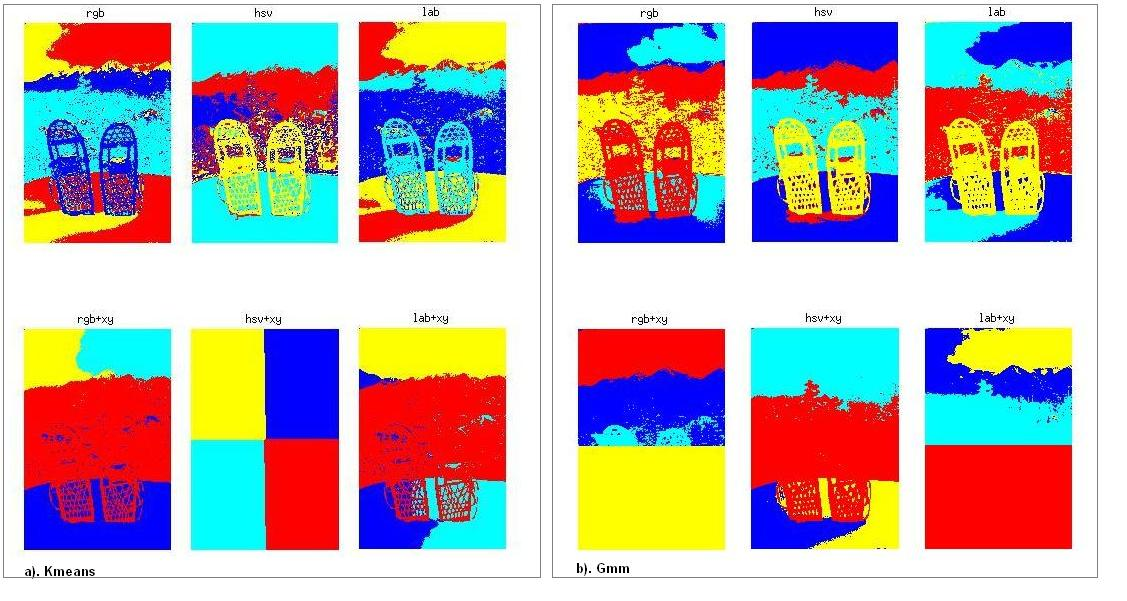
\includegraphics[scale=0.3]{pru.JPG}
\end{center}
   \caption{kmeans y espacios de color para K=4 }
\label{fig:long}
\label{fig:onecol}
\end{figure}

se encontró que en la implementación de las técnicas como k-means y gmm para los espacios de colorque tienen encuenta la ubicación del x,y del píxel no muestra buenos Resultados 
a pesar de que se creía que el tener en cuenta la relación con los vecinos la segmentación iba a ser mejor. al analizar estos resulados y la manera en como se propúso la metodología,
es posible afirmar que al realizar el cambio en ubicación espacial de la imagen y convertirlo en en una matriz 2D con 5 variables de clasificación(primer, segundo y tercer componente del espacio de color, eje x y eje y)
las dos variables de posición son muy significativas para la clasificación. 

\subsection{Métodos de segmentación}

en  los métodos de segmentac
kmeans y gmm como algoritmos de clusteringa grupan según un k dado, en la metodolosá propuesta se evaluó otro métodos
el watershed que como se puede observar en la figura xx presentó una sobre segmentación y al incrementar el h para el
nivel de los mínimos regionales la sobre segmentación disminuye pero no queda la imagen bien segmentada, dado que esta
imágen depende de la luminosidad para definir los niveles de altitud del relieve. 

en cuanto a kmenas y gmm es dificil evaluar visualmente cuál tiene un mejor funcionamiento en la segmentación de las imágenes 
digitales.
\begin{figure}[t]
\begin{center}
\fbox{\rule{0pt}{2in} \rule{0.8\linewidth}{0pt}
    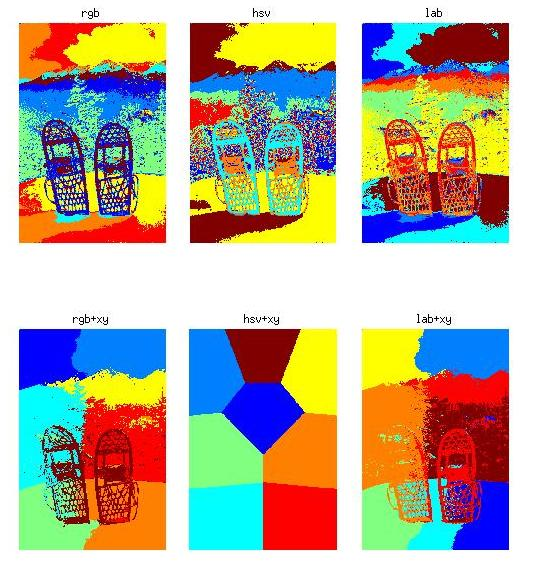
\includegraphics[width=0.8\linewidth]{seg1_k-means8.jpg}}
\end{center}
    \caption{Segmentaci\'on por k-means para k=8 en los espacios rgb, hsv y lab incluyendo las posiciones p\'ixeles}
\label{fig:long}
\label{fig:onecol}
\end{figure}
 

es dificil decir que espacio de reprentación es el mejor para cada técnica de clasificación.
para ello se realizó una comprobación de los métodos de segmentación propuestos, mediante la 
Evalución


\subsection{Evalución}

los resultados de segmentación incluyendo coordenadas no mejoran la clasificaión.


\section{Discusión}

%-------------------------------------------------------------------------
\subsection{References}

% \
% 
% \begin{table}
% \begin{center}
% \begin{tabular}{|l|c|}
% \hline
% Method & Frobnability \\
% \hline\hline
% Theirs & Frumpy \\
% Yours & Frobbly \\
% Ours & Makes one's heart Frob\\
% \hline
% \end{tabular}
% \end{center}
% \caption{Results.   Ours is better.}
% \end{table}
% 
% %-------------------------------------------------------------------------
% \subsection{Illustrations, graphs, and photographs}
% 
% \begin{figure}[t]
% \begin{center}
%    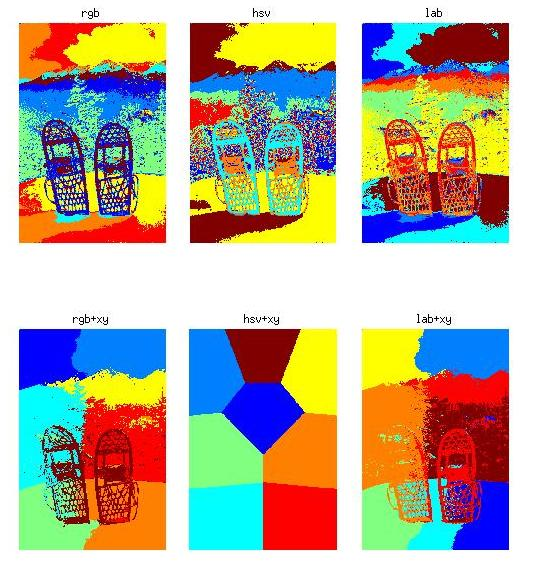
\includegraphics[width=0.8\linewidth]{seg1_k-means8.jpg}
% \end{center}
%    \caption{Segmentaci\'on por k-means para k=8 en los espacios rgb, hsv y lab incluyendo las posiciones p\'ixeles}
% \label{fig:long}
% \label{fig:onecol}
% \end{figure}
% 
% \begin{figure}[t]
% \begin{center}
%    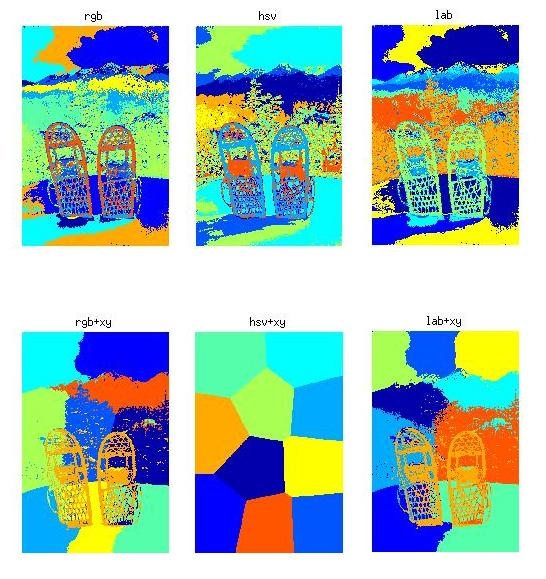
\includegraphics[width=0.8\linewidth]{seg1_k-means10.jpg}
% \end{center}
%    \caption{Segmentaci\'on por k-means para k=10 en los espacios rgb, hsv y lab incluyendo las posiciones p\'ixeles}
% \label{fig:long}
% \label{fig:onecol}
% \end{figure}
% 
% \begin{figure}[t]
% \begin{center}
%    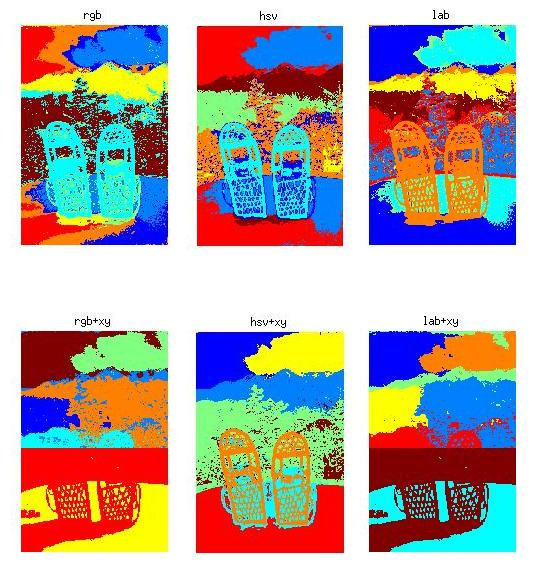
\includegraphics[width=0.8\linewidth]{seg2_gmm8.jpg}
% \end{center}
%    \caption{Segmentaci\'on por gmm para k=8 en los espacios rgb, hsv y lab incluyendo las posiciones p\'ixeles}
% \label{fig:long}
% \label{fig:onecol}
% \end{figure}
% 
% \begin{figure}[t]
% \begin{center}
%    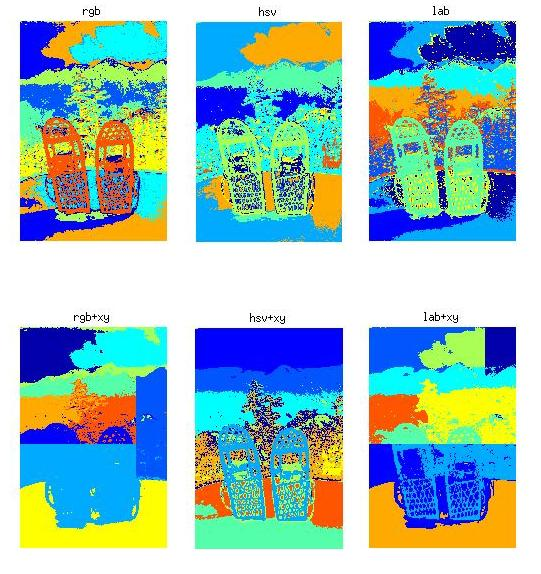
\includegraphics[width=0.8\linewidth]{seg2_gmm10.jpg}
% \end{center}
%    \caption{Segmentaci\'on por gmm para k=10 en los espacios rgb, hsv y lab incluyendo las posiciones p\'ixeles{}
% \label{fig:long}
% \label{fig:onecol}
% \end{figure}


%------------------------------------------------------------------------
\section{Final copy}


{\small
\bibliographystyle{apalike}
\bibliography{ref1.bib}


\end{document}
